\section{DefineLanguage: Non-Terminal Cycle Checking}

\subsection{Motivation}
PltRedex doesn't allow language definitions such as the one in Figure \ref{dl-ntcyclegraph}.

\begin{figure}[H]
\begin{minipage}{0.45\linewidth}
	\centering
\begin{minted}[tabsize=1,obeytabs,escapeinside=||,mathescape=true,linenos,fontsize=\small]{racket}
(define-language L
	(e ::= (e e) n)
	(n ::= (n n) number p)
	(p ::= (p p) real e))
	(s ::= string)
\end{minted}
\end{minipage}
\begin{minipage}{0.45\linewidth}
	\centering
	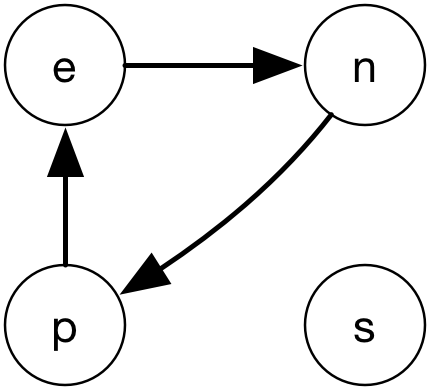
\includegraphics[scale=0.18]{transformation-pattern-ntgraph.png}
\end{minipage}
	\caption{\texttt{define-language} and its non-terminal graph}
	\label{dl-ntcyclegraph}
\end{figure}

The problem with the language above (aside from it being completely useless) is a cycle of non-terminals $n \rightarrow p \rightarrow e$. When testing if some term is a non-terminal, a term is matched against every pattern in a non-terminal definition. For example, given term \texttt{String("hello world")}, it is matched against non-terminal \texttt{e}. Since  the term doesn't match the pattern \texttt{(e e)}, non-terminal \texttt{n} is then matched. Since the term doesn't match any patterns here either, non-terminal \texttt{p} is then matched. Similarly, the term doesn't match any patterns here either, \texttt{e} is then matched, but that's where the matching has started and thus \textit{infinite recursion} becomes an issue. Languages need to be analyzed for presence of non-terminal cycles.

\subsection{Algorithm}
To detect such cycles, \DefineLanguageNoArg \space needs to be interpreted as a directed graph and some cycle-detecting algorithm must be used. The graph is constructed in the following manner.

\begin{enumerate}
\item
For each \NtDefinitionN[n], create a vertex labeled $n$.
\item
For $p_1, ..., p_n$, if $p_i$ is \NtDefinitionN[m], create the edge $n\rightarrow m$.
\end{enumerate}


To detect cycles, depth-first-search is employed. Vertices in the graph can be assigned one of three colors:

\begin{itemize}
\item

\textbf{White} - meaning the vertex hasn't been visited before. All vertices are initially assigned this color.

\item
\textbf{Gray} - meaning successors of the vertex $v$ are still being visited. When $v$ is visited for the first time, $color(v)$ becomes \textbf{Gray}.
\item
\textbf{Black} - meaning all successors of the vertex $v$ have been explored.
\end{itemize}



The detection of cycles is done through vertex coloring. For example, if during depth-first-traversal vertex $v$ is encountered with \DFSColor{$v$}{Gray}, this means that there's a \textbf{back-edge} in the tree created by depth-first traversal. That is, back-edge $u \rightarrow v$ connects vertex $u$ to its predecessor in the depth-first-search tree $v$. Once such cycle is found, the error is reported and the compilation aborts.

To report a path of non-terminals that make up the cycle, a path of non-terminals has to be maintained. The path can be represented as a stack. Given starting vertex $v$, depth-first-search proceeds as follows:

\begin{enumerate}
\item If \DFSColor{$v$}{Gray}, report cycle and abort compilation.
\item If \DFSColor{$v$}{White}, set color to \textbf{Gray} and add $v$ to the path.
\item Visit each successor vertex $v^{\prime}$ recursively.
\item Set color of $v$ to \textbf{Black} and remove it from the path.
\end{enumerate}

Since the resulting non-terminal graphs may be disjoint, we need to keep track of visited vertices during traversal. Let $V$ be a set of vertices whose \DFSColor{$v$}{Black}. Thus, every time vertex $v$ changes its color to \textbf{Black}, $V = V \cup \{v\} $. Let $U$ be a set of vertices whose \DFSColor{$v$}{White}; that is, it initially contains all the non-terminals. The algorithm proceeds as follows:

\begin{enumerate}
\item
Pick a random vertex $u$ from set $U$. Create empty set $V$. Starting from $u$, perform depth-first-search as described above. Compute set difference - $U = U-V$.
\item
Continue until $U$ is empty.
\end{enumerate}

It should be noted that the algorithm described does not report all the cycles in the graph but the first one it manages to find. One improvement could be finding all cycles in the graph.

\subsection{Example}

Figure \ref{nt-cycle-example} demonstrates cycle searching using the graph shown in Figure \ref{dl-ntcyclegraph} starting from the non-terminal $s$. Initially $U=\{s,p,n,e\}$. Its color becomes \texttt{Gray} as seen in (a). Since it has no successor vertices, its color becomes \texttt{Black}, as seen in (b).

Since $V = \{ s \}$, $U=\{p,n,e\}$. Pick vertex $p$ for expansion and color it \texttt{Gray}. Then, visit the only successor of $s$, vertex $e$ and color it \texttt{Gray}. Visit the only successor of $e$, vertex $n$ and color it \texttt{Gray}. Finally, visit the only successor of $n$, vertex $p$. But since it is already colored \texttt{Gray}, the cycle  $p \rightarrow e \rightarrow n$ has been found and a compilation error should be raised.

\begin{figure}[h]
\begin{subfigure}{0.32\linewidth}
	\centering
	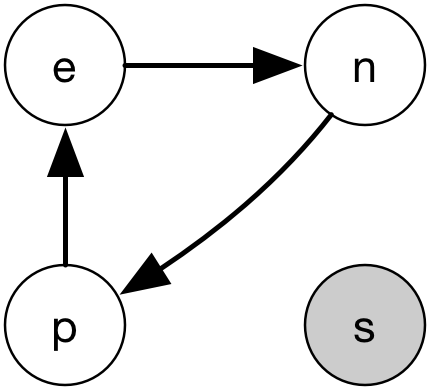
\includegraphics[scale=0.18]{transformation-pattern-ntgraph-example-1.png}
\end{subfigure}
\begin{subfigure}{0.32\linewidth}
	\centering
	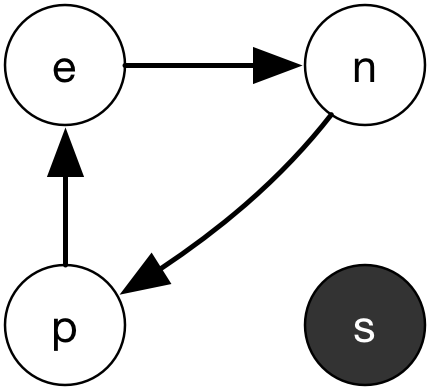
\includegraphics[scale=0.18]{transformation-pattern-ntgraph-example-2.png}
\end{subfigure}
\begin{subfigure}{0.32\linewidth}
	\centering
	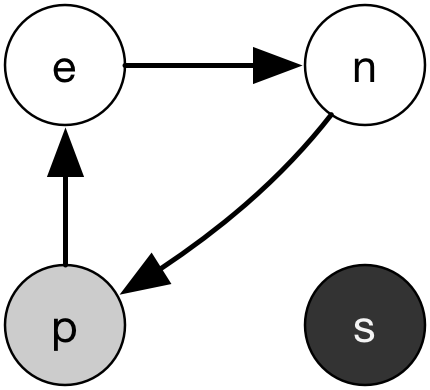
\includegraphics[scale=0.18]{transformation-pattern-ntgraph-example-3.png}
\end{subfigure}
\newline
\begin{subfigure}{0.32\linewidth}
	\centering
	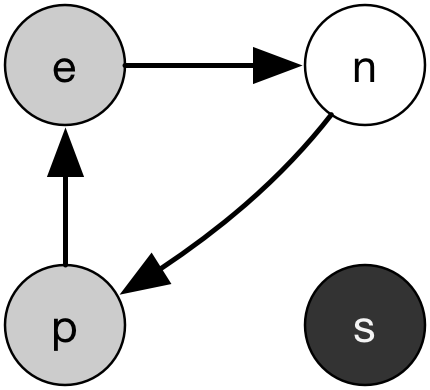
\includegraphics[scale=0.18]{transformation-pattern-ntgraph-example-4.png}
\end{subfigure}
\begin{subfigure}{0.32\linewidth}
	\centering
	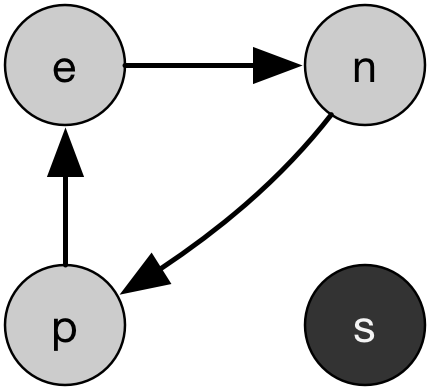
\includegraphics[scale=0.18]{transformation-pattern-ntgraph-example-5.png}
\end{subfigure}
\begin{subfigure}{0.32\linewidth}
	\centering
	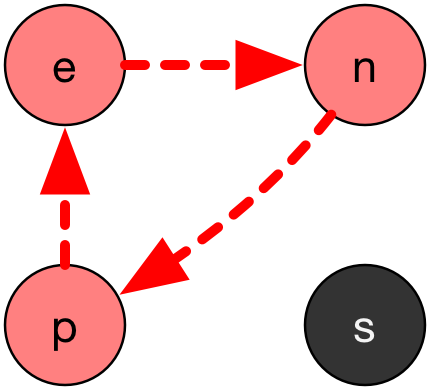
\includegraphics[scale=0.18]{transformation-pattern-ntgraph-example-6.png}
\end{subfigure}
\caption{Cycle searching using DFS.}
\label{nt-cycle-example}
\end{figure}
